\documentclass[11pt,a4paper]{ctexart}

\usepackage[a4paper,margin=1in]{geometry}
\usepackage[colorlinks=true,linkcolor=blue,urlcolor=blue,citecolor=blue]{hyperref}
\usepackage{booktabs}
\usepackage{longtable}
\usepackage{array}
\usepackage{tabularx}
\usepackage{graphicx}
\usepackage{float}
\usepackage{enumitem}
\usepackage{xurl}
\usepackage{setspace}

\title{TransChromBP 阶段报告与论文主线重构\\
\large 从 tutorial 结果汇总转向 Transformer、蒸馏与 bias 机制研究}
\author{项目工作文档}
\date{2026 年 3 月 15 日}

\begin{document}

\maketitle
\onehalfspacing

\begin{abstract}
本文档不再只是此前 tutorial 评估、hybrid\_data 审计和推荐数据处理流程的汇编，而是
在保留这些结果的同时，重新定义 TransChromBP 的论文主线。当前阶段已经建立了三条稳定结论：
第一，原始 \texttt{bias\_pretrain -> main\_learnable} 主线在 held-out
\texttt{test(chr1)} 上优于 tutorial baseline，可作为可信起点。第二，\texttt{hybrid\_data}
更适合作为一次数据语义负对照，而不是新的默认训练线；它没有证明原始主线建立在明显错误的
数据处理上。第三，ATAC 专用数据语义已经足够清晰，后续论文不应继续围绕它作为主战场。
基于此，本文把研究目标正式收敛为一个更强的问题：在碱基分辨率 ATAC-seq profile prediction
中，AlphaGenome 式的 Transformer 长程建模与 teacher-student distillation，和
ChromBPNet 式的 bias factorization，究竟分别起什么作用、如何交互，以及能否在同一旗舰模型中
共同带来更强结果。文中给出新的论文叙事、旗舰模型定义、实验矩阵、当前证据与固定约束条件，
并保留后续复现所需的关键路径与资产目录。
\end{abstract}

\section{为什么要重构主线}

此前这条工作线已经积累了足够多的结果，但它们原本分散在三类叙事里：
\begin{itemize}[leftmargin=2em]
  \item tutorial 主线是否优于 baseline；
  \item hybrid\_data 是否说明数据处理存在明显偏差；
  \item 推荐数据处理流程应如何参考 ChromBPNet 和 AlphaGenome。
\end{itemize}

这些问题在项目推进早期都合理，但继续围绕它们组织全文，会使论文主线停留在
“哪套 recipe 更像正确做法”的层面。当前证据已经足以让我们把这个阶段收束成前提条件，
并把论文真正的问题上移到机制层：
\begin{quote}
在 ATAC 碱基分辨率建模中，Transformer、distillation 与 ChromBPNet-style bias
factorization 的作用关系是什么。
\end{quote}

\section{当前已经确定的事实}

\subsection{事实一：当前主线优于 baseline}

在独立 held-out \texttt{test(chr1)} 的 \texttt{62342} 个 region 上，原始主线与
tutorial baseline 的关键结果如下。

\begin{table}[H]
\centering
\small
\begin{tabular}{lrrrrrr}
\toprule
模型 & overall $r$ & overall JSD & peak $r$ & peak JSD & nonpeak $r$ & nonpeak JSD \\
\midrule
\texttt{Orig best} & 0.8416 & 0.4455 & 0.8207 & 0.3310 & 0.2276 & 0.5599 \\
\texttt{Orig epoch20} & 0.8347 & 0.4428 & 0.8141 & 0.3276 & 0.2359 & 0.5581 \\
\texttt{Baseline epoch20} & 0.8253 & 0.4536 & 0.8048 & 0.3437 & 0.1875 & 0.5635 \\
\bottomrule
\end{tabular}
\caption{当前可信主线与 tutorial baseline 的 held-out test 对比。}
\end{table}

这一定义了后续工作的固定起点：
\begin{itemize}[leftmargin=2em]
  \item \texttt{Orig best} 代表 peak-first checkpoint；
  \item \texttt{Orig epoch20} 代表 overall-balanced checkpoint；
  \item tutorial baseline 不再是后续自研模型的首选主参照。
\end{itemize}

\begin{figure}[H]
\centering
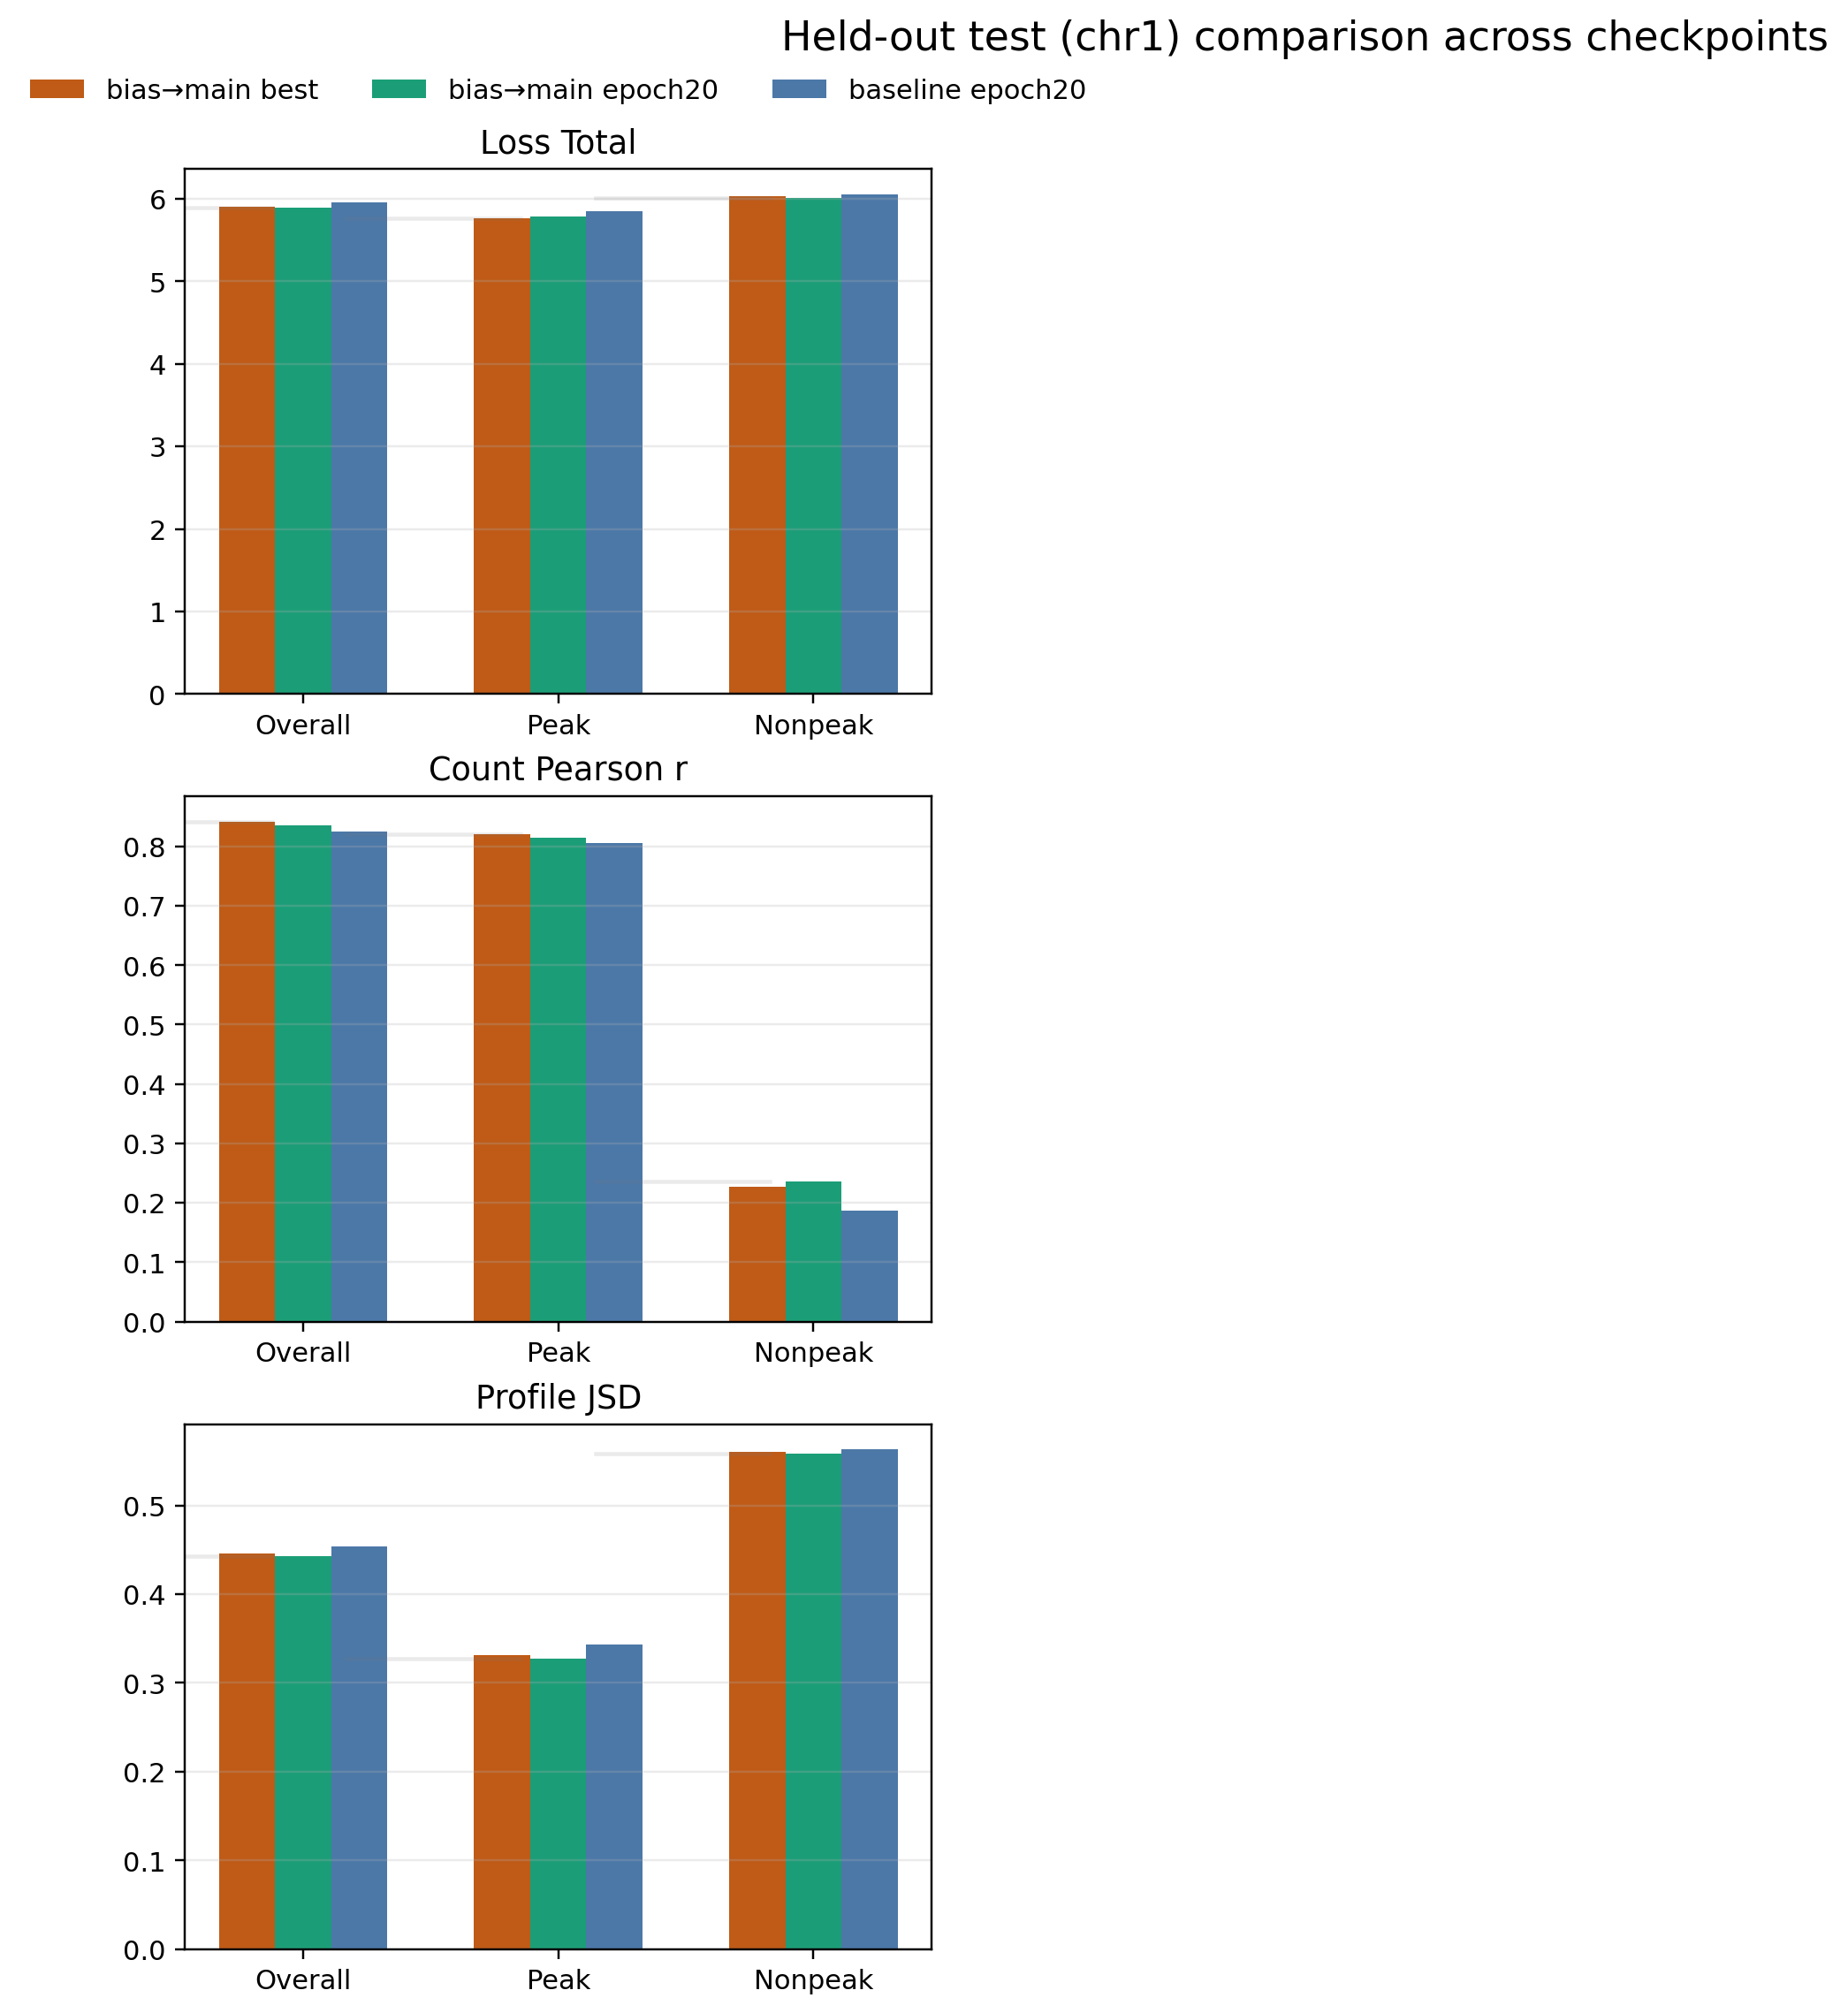
\includegraphics[width=0.72\linewidth]{assets/transchrombp_tutorial_test_20260315/figures/test_metric_comparison.png}
\caption{tutorial 主线与 baseline 的 held-out test 主指标对比。}
\end{figure}

\subsection{事实二：hybrid\_data 是一次有价值的负对照}

\texttt{hybrid\_data} 同时把 peak-only jitter、moderate nonpeak exposure、
automatic count calibration 和在线 track-depth scaling 绑在了一起。它的结果更适合被理解为：
\begin{quote}
“把多项来自 ChromBPNet 和 AlphaGenome 的启发整包照搬”并不会自然得到更好的 ATAC 主线。
\end{quote}

在 full held-out test 上，它没有超过原始主线：

\begin{table}[H]
\centering
\small
\begin{tabular}{lrr}
\toprule
模型 & overall $r$ & overall JSD \\
\midrule
\texttt{Orig epoch20} & 0.8347 & 0.4428 \\
\texttt{Hybrid learnable epoch20} & 0.8000 & 0.4703 \\
\texttt{Hybrid fixed epoch20} & 0.7946 & 0.4687 \\
\bottomrule
\end{tabular}
\caption{原始主线与 hybrid 主线在 full held-out test 上的总体对比。}
\end{table}

在 trimmed test 上，排名也没有翻转。这个结果的意义不是“数据处理不重要”，而是：
\begin{itemize}[leftmargin=2em]
  \item 当前项目没有被明显错误的数据语义卡死；
  \item 数据语义应作为固定前提，而不是继续做论文主角；
  \item 之后如果还改数据语义，应服务于模型主线，而不是重新定义问题。
\end{itemize}

\begin{figure}[H]
\centering
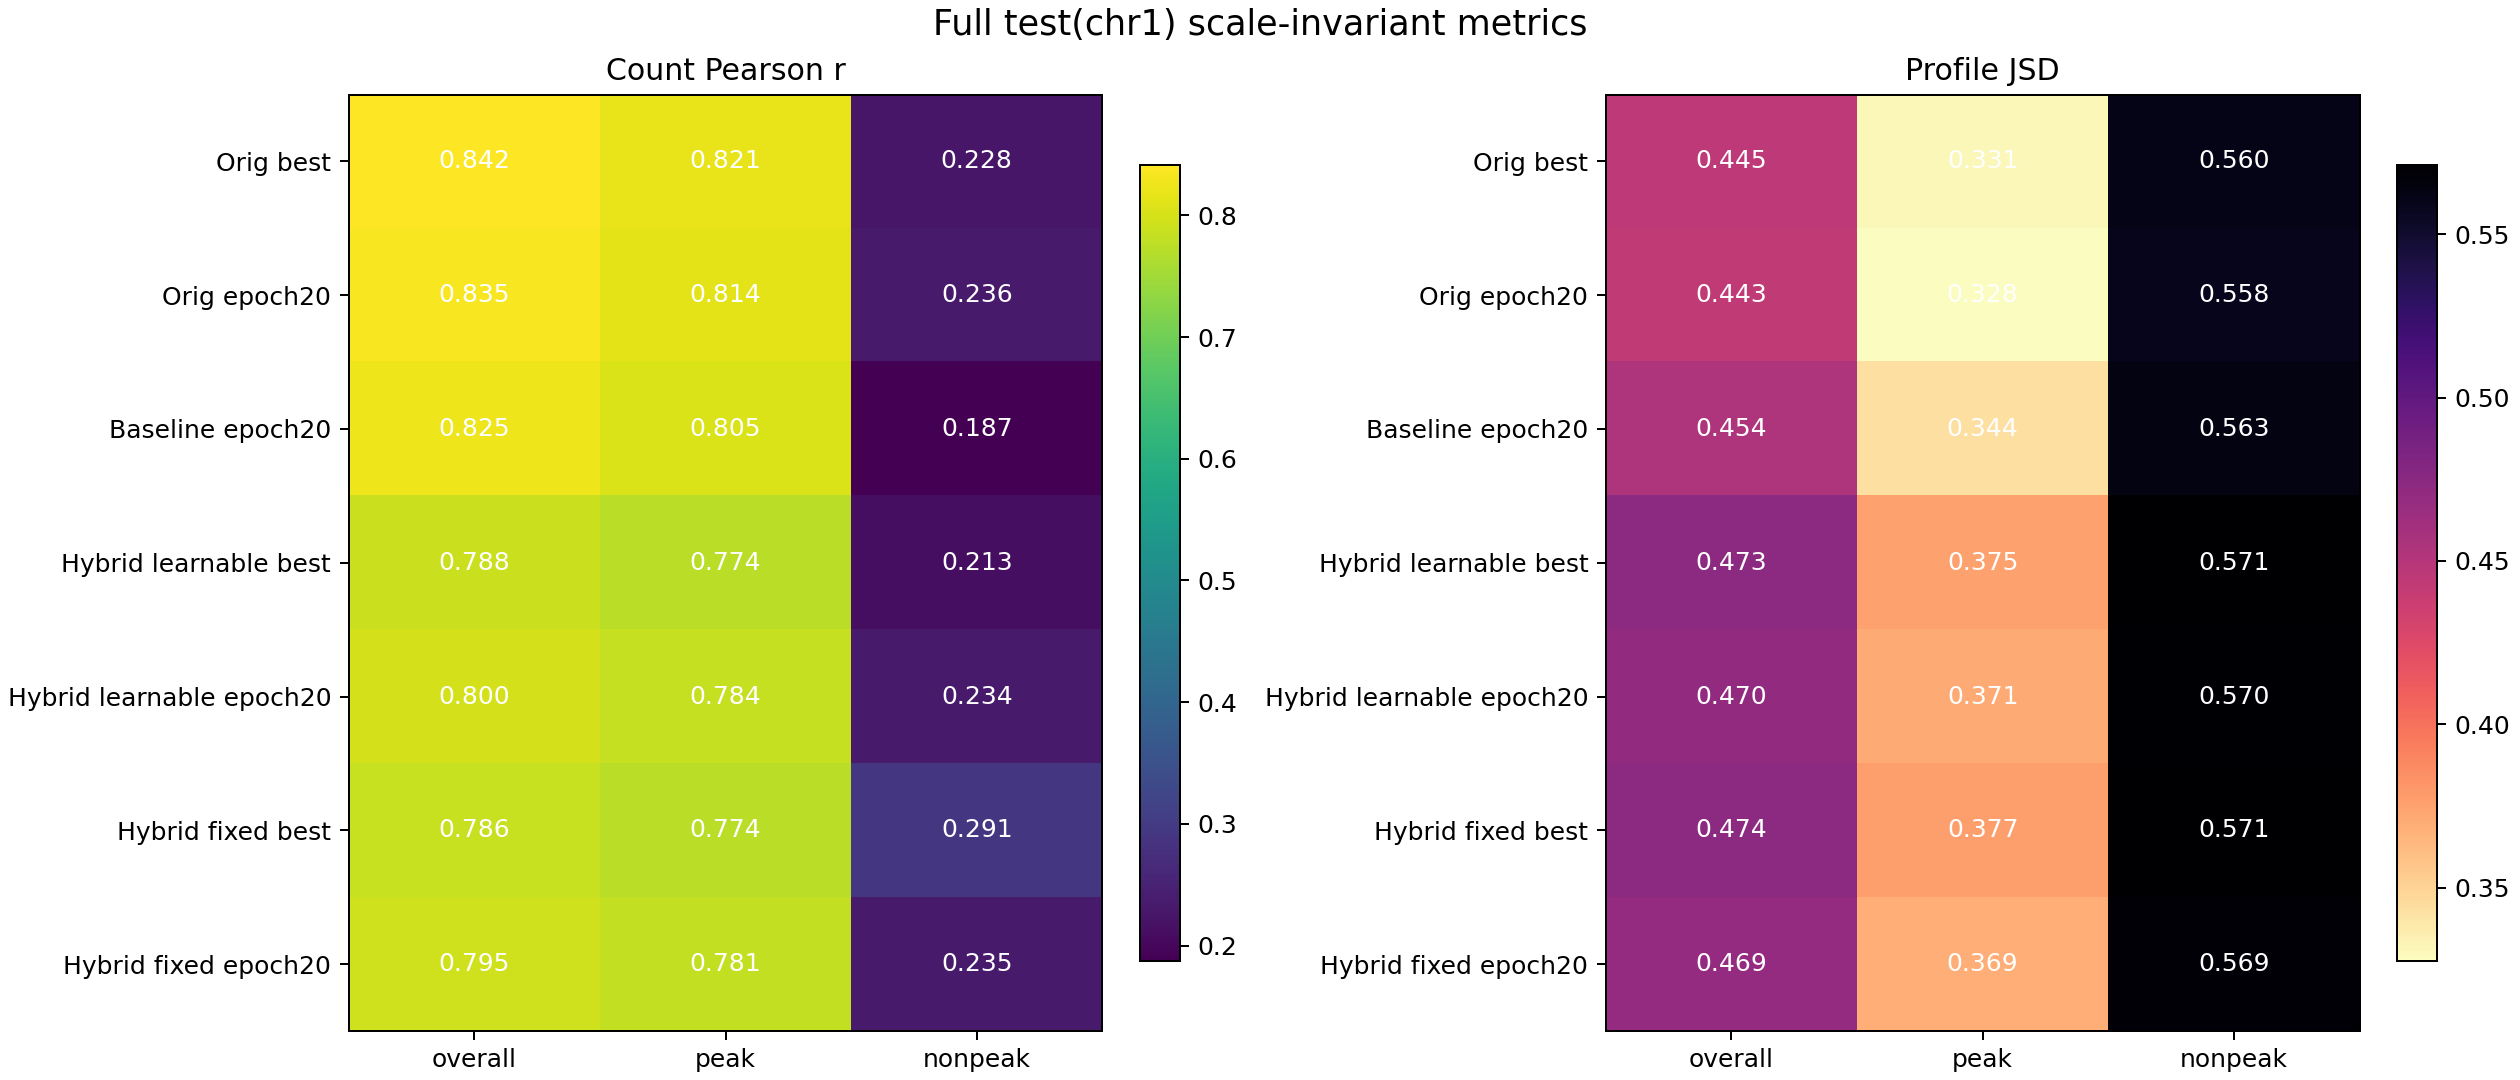
\includegraphics[width=\linewidth]{assets/transchrombp_hybrid_eval_20260315/figures/full_test_scale_invariant_heatmaps.png}
\caption{hybrid\_data 审计结果热图。它说明当前更适合作为负对照，而不是新主线。}
\end{figure}

\subsection{事实三：bias branch 具备独立职责}

bias-only sanity check 已经说明，background bias 本身是可学对象，但不应在 peak 上承担主任务。

\begin{table}[H]
\centering
\small
\begin{tabular}{lrrr}
\toprule
bias 模型 & split & count $r$ & profile JSD \\
\midrule
\texttt{Orig bias\_pretrain} & peak & -0.0089 & 0.4002 \\
\texttt{Orig bias\_pretrain} & nonpeak & 0.4633 & 0.5685 \\
\texttt{Hybrid bias\_pretrain} & peak & 0.1823 & 0.4016 \\
\texttt{Hybrid bias\_pretrain} & nonpeak & 0.5412 & 0.5692 \\
\bottomrule
\end{tabular}
\caption{bias-only sanity check。}
\end{table}

这为后续论文提供了一个重要边界：讨论 Transformer 和 distillation 之前，必须保留
bias-aware task formulation，否则很难判断模型到底是在学调控结构，还是在学实验偏差。

\section{新的论文主线}

\subsection{从“recipe 争论”转向“机制交互”}

新的论文主线不再是：
\begin{quote}
哪一种数据处理流程更像正确答案。
\end{quote}

而是：
\begin{quote}
在 ATAC 碱基分辨率 profile prediction 中，Transformer 长程建模、teacher-student
distillation 和 ChromBPNet-style bias factorization 究竟如何共同作用。
\end{quote}

这一定义的好处是，它既保留了 ChromBPNet 的任务清晰性，也吸收了 AlphaGenome 真正值得学的部分，
但不会把论文写成一个不必要的多模态 foundation model。

\subsection{论文要同时完成两件事}

这篇论文必须同时满足两个目标：
\begin{enumerate}[leftmargin=2em]
  \item 提出一个足够强、可以冲击 benchmark 最优结果的旗舰模型；
  \item 围绕这个旗舰模型，系统分析三类机制的作用与交互。
\end{enumerate}

缺任何一个都不够。只有强模型没有机制解释，会显得像单纯堆模型；只有机制分析没有强主结果，
又会显得像“因为模型不够强，所以只能做分析”。

\section{旗舰模型定义}

\subsection{推荐的旗舰模型}

论文主模型建议定义为：
\begin{quote}
\textbf{Teacher-Student TransChromBP}：
卷积 stem + compressed-token Transformer + ChromBPNet-style bias branch +
profile/count 双头 + knowledge distillation。
\end{quote}

它的核心组成应包括：
\begin{itemize}[leftmargin=2em]
  \item 卷积 stem：负责 motif 级局部结构；
  \item 主干 Transformer：负责较长距离上下文；
  \item bias branch：负责 assay-specific 偏差；
  \item fusion 模块：组合 debiased prediction 与 bias correction；
  \item teacher / student：teacher 更强，student 更轻，二者共享相同任务语义。
\end{itemize}

\subsection{为什么 distillation 是必须项}

没有蒸馏时，Transformer 的收益很容易被读成“更大的模型更强”。一旦加入 teacher-student
结构，问题才会变得更有内容：
\begin{itemize}[leftmargin=2em]
  \item teacher 学到的长程知识是否可迁移；
  \item 迁移后 student 的收益落在 profile、count、peak 还是 nonpeak；
  \item 蒸馏后的 student 是否仍然需要 bias factorization；
  \item 如果没有 bias branch，蒸馏收益会不会被错误地吸收到 bias 中。
\end{itemize}

\subsection{固定前提：数据语义不再是主变量}

后续实验都应建立在固定的 ATAC 专用数据语义上：
\begin{itemize}[leftmargin=2em]
  \item shifted unstranded insertion bigWig；
  \item peak-centered windows；
  \item GC-matched nonpeaks；
  \item bias 预训练使用 nonpeak-only、no jitter；
  \item main 训练使用 peak-centric supervision 和较低 nonpeak exposure；
  \item train-only reverse-complement augmentation；
  \item automatic count loss calibration。
\end{itemize}

\section{实验程序应如何围绕新主线组织}

\subsection{三条核心实验轴}

后续实验不宜再铺一个很大的全因子矩阵，而应围绕三条主轴：
\begin{itemize}[leftmargin=2em]
  \item \textbf{Backbone axis}: conv-only vs conv+Transformer；
  \item \textbf{Training axis}: direct training vs distillation；
  \item \textbf{Bias axis}: no bias vs fixed bias vs learnable bias。
\end{itemize}

\subsection{主结果表最小必要集合}

主结果表建议包含：
\begin{enumerate}[leftmargin=2em]
  \item ChromBPNet / 当前 conv-only 强基线；
  \item Student TransChromBP（无 distillation）；
  \item Student TransChromBP（有 distillation）；
  \item Transformer + bias、无 distillation；
  \item Transformer + distillation、无 bias；
  \item Full flagship：Transformer + distillation + learnable bias；
  \item Full flagship：Transformer + distillation + fixed bias。
\end{enumerate}

\subsection{解释和分层分析}

如果论文要站得住，不能只看 aggregate 指标。至少应补：
\begin{itemize}[leftmargin=2em]
  \item peak / nonpeak 分层结果；
  \item full output 与 debiased output 的分开评估；
  \item bias scale / fusion 轨迹；
  \item locus-level 轨道图；
  \item 若条件允许，SHAP / motif / MoDISco；
  \item 若实现成熟，再补 ATAC-specific scorer。
\end{itemize}

\section{这份阶段报告对后续论文的意义}

当前结果并不是论文终点，而是论文起点。它们已经帮我们完成了三件关键事情：
\begin{enumerate}[leftmargin=2em]
  \item 确定了一个可信的起始模型主线；
  \item 把数据语义问题降级为固定约束，而不是继续做中心矛盾；
  \item 证明 bias branch 确实是一个值得保留和分析的任务组件。
\end{enumerate}

因此，后续所有正式实验和写作都应接受同一个判断标准：
\begin{quote}
它是否有助于强化旗舰模型，或者更清楚地解释 Transformer、distillation 与 bias factorization
 的关系。
\end{quote}

\section{关键保留路径}

\subsection*{本地报告与骨架}
\begin{itemize}[leftmargin=2em]
  \item \texttt{reports/transchrombp\_tutorial\_consolidated\_cn.tex}
  \item \texttt{reports/transchrombp\_tutorial\_consolidated\_cn.pdf}
  \item \texttt{reports/transchrombp\_paper\_outline\_cn.tex}
  \item \texttt{reports/transchrombp\_paper\_outline.tex}
  \item \texttt{reports/transchrombp\_project\_note\_cn.tex}
\end{itemize}

\subsection*{关键资产目录}
\begin{itemize}[leftmargin=2em]
  \item \texttt{reports/assets/transchrombp\_tutorial\_test\_20260315/}
  \item \texttt{reports/assets/transchrombp\_hybrid\_eval\_20260315/}
  \item \texttt{reports/assets/transchrombp\_recommended\_data\_semantics\_20260315/}
\end{itemize}

\subsection*{远端冻结快照}
\begin{itemize}[leftmargin=2em]
  \item \texttt{/data1/zhoujiazhen/bylw\_atac/TransChromBP/outputs/snapshots/tutorial\_report\_20260315\_frozen/}
  \item \texttt{/data1/zhoujiazhen/bylw\_atac/TransChromBP/outputs/snapshots/data\_semantics\_audit\_20260315\_frozen/}
\end{itemize}

大权重仍只保留在远端，不下载回本地；本地文档负责描述它们的路径与作用。

\end{document}
